\documentclass[12pt]{article}

\usepackage[margin=1.9cm, letterpaper]{geometry}
\usepackage{fontspec}
\usepackage{mathtools}
\usepackage{pgfplots}
\usepackage{siunitx}
\usepackage{subcaption}
\usepackage{graphicx}
\usepackage{makecell}
\usepackage{float}

\pgfplotsset{compat=newest}

\title{EXPERIMENT 4: \protect\\Magnetic Fields}
\date{March 12, 2019}
\author{Michael Kwok | Partner: Cyrus Diego }

\begin{document}
\maketitle
\pagebreak

\section{Introduction}
In this experiment, the relationship between electric currents and magnetic
fields will be observed. This relationship was first discovered by Hans
Christian Oersted in the 1800s, where he noticed that a wire with an electric
current flowing through it caused a deflection on a compass. He came up with the
following equation for the magnetic field $\Delta B$ by a tiny segment of coil $\Delta l$:

\begin{equation} \label{eq:deltaB}
    \Delta B = \frac{\mu_0I\Delta l \sin\theta}{4\pi r^2}
\end{equation}

where $\mu_0$ is the constant of permeability of free space, $I$ is the current
in the wire, $\theta$ is the angle between the segment and the displacement, and
$r$ is the current displacement.

The Hall effect is when a potential difference is produced in a conductor due to a
current passing in the conductor while within a magnetic field. It was discovered
by Edwin hall in 1879.

We will also be using a solenoid, which is a tightly wound coil of wire. This coil
of wire produces a uniform magnetic field when current is passing through the
wire. The equation for the magnetic field in the central axis of a solenoid is given as:

\begin{equation} \label{eq:B}
    B = \frac{1}{2}\mu_0nI(\cos\beta_2-\cos\beta_1)
\end{equation}

where $n = N/L$, the number of turns per unit length of the solenoid, and $\beta_1$
and $\beta_2$ are angles between the sides and the center of the solenoid from
the displacement respectively.

A Helmholtz coil is used in the second part of the experiment. This coil is similar
to the solenoid. However, it has two sets of coils a set distance apart, and the entire
volume between the two coils will have a homogenous magnetic field. The magnetic field
in the center of the two coils is given as the following:

\begin{equation} \label{eq:B_Helmholtz}
    B_H = \frac{8\mu_0NI}{\sqrt{125}R}
\end{equation}
where $N$ is the number of turns in the coil, $I$ is the current, $R$ is the coil's
radius.

We will be determining the distribution of the magnetic field along the axis of the solenoid,
and the magnetic field of the Helmholtz coil, getting the number of turns of the coil
afterwards.

\section{Methods}
\subsection*{Part 1}
\begin{itemize}
    \item Wire up the $+$ terminal of a DC power supply to a switch, then wire the switch
          to the solenoid. Connect the other end of the solenoid to the DC power supply.
          Keep the circuit open.

    \item Set up a Hall effect probe to collect the data from. Record the ambient magnetic
          field $B_e$.

    \item Close the circuit, then set the current on the power supply to be \SI{1.0}{\volt}.
          Ensure magnetic fields are positive. If not, flip the polarity of the leads.

    \item Slide the probe along the length of the solenoid, recording the field strength
          measurements every 2 cm.

    \item Take down the length $L$, radius $R$, number of turns $N$, and the midpoint ruler
          position $x_c$ of the solenoid.
\end{itemize}

\subsection*{Part 2}
\begin{itemize}
    \item Connect the two Helmholtz coils to be in series with the DC Power source,
          just like the previous part.

    \item Carefully position the tip of the Hall effect probe to the center of the two
          coils.

    \item Record the measured field strength at \SI{0.1}{\ampere} intervals between \SI{0.1}{\ampere}
          and \SI{1.0}{\ampere}.
\end{itemize}
\section{Results}
The results collected are as follows (See also \ref{fig:part1_results} and \ref{fig:part2_results} in appendix):
\begin{figure}[!ht]
    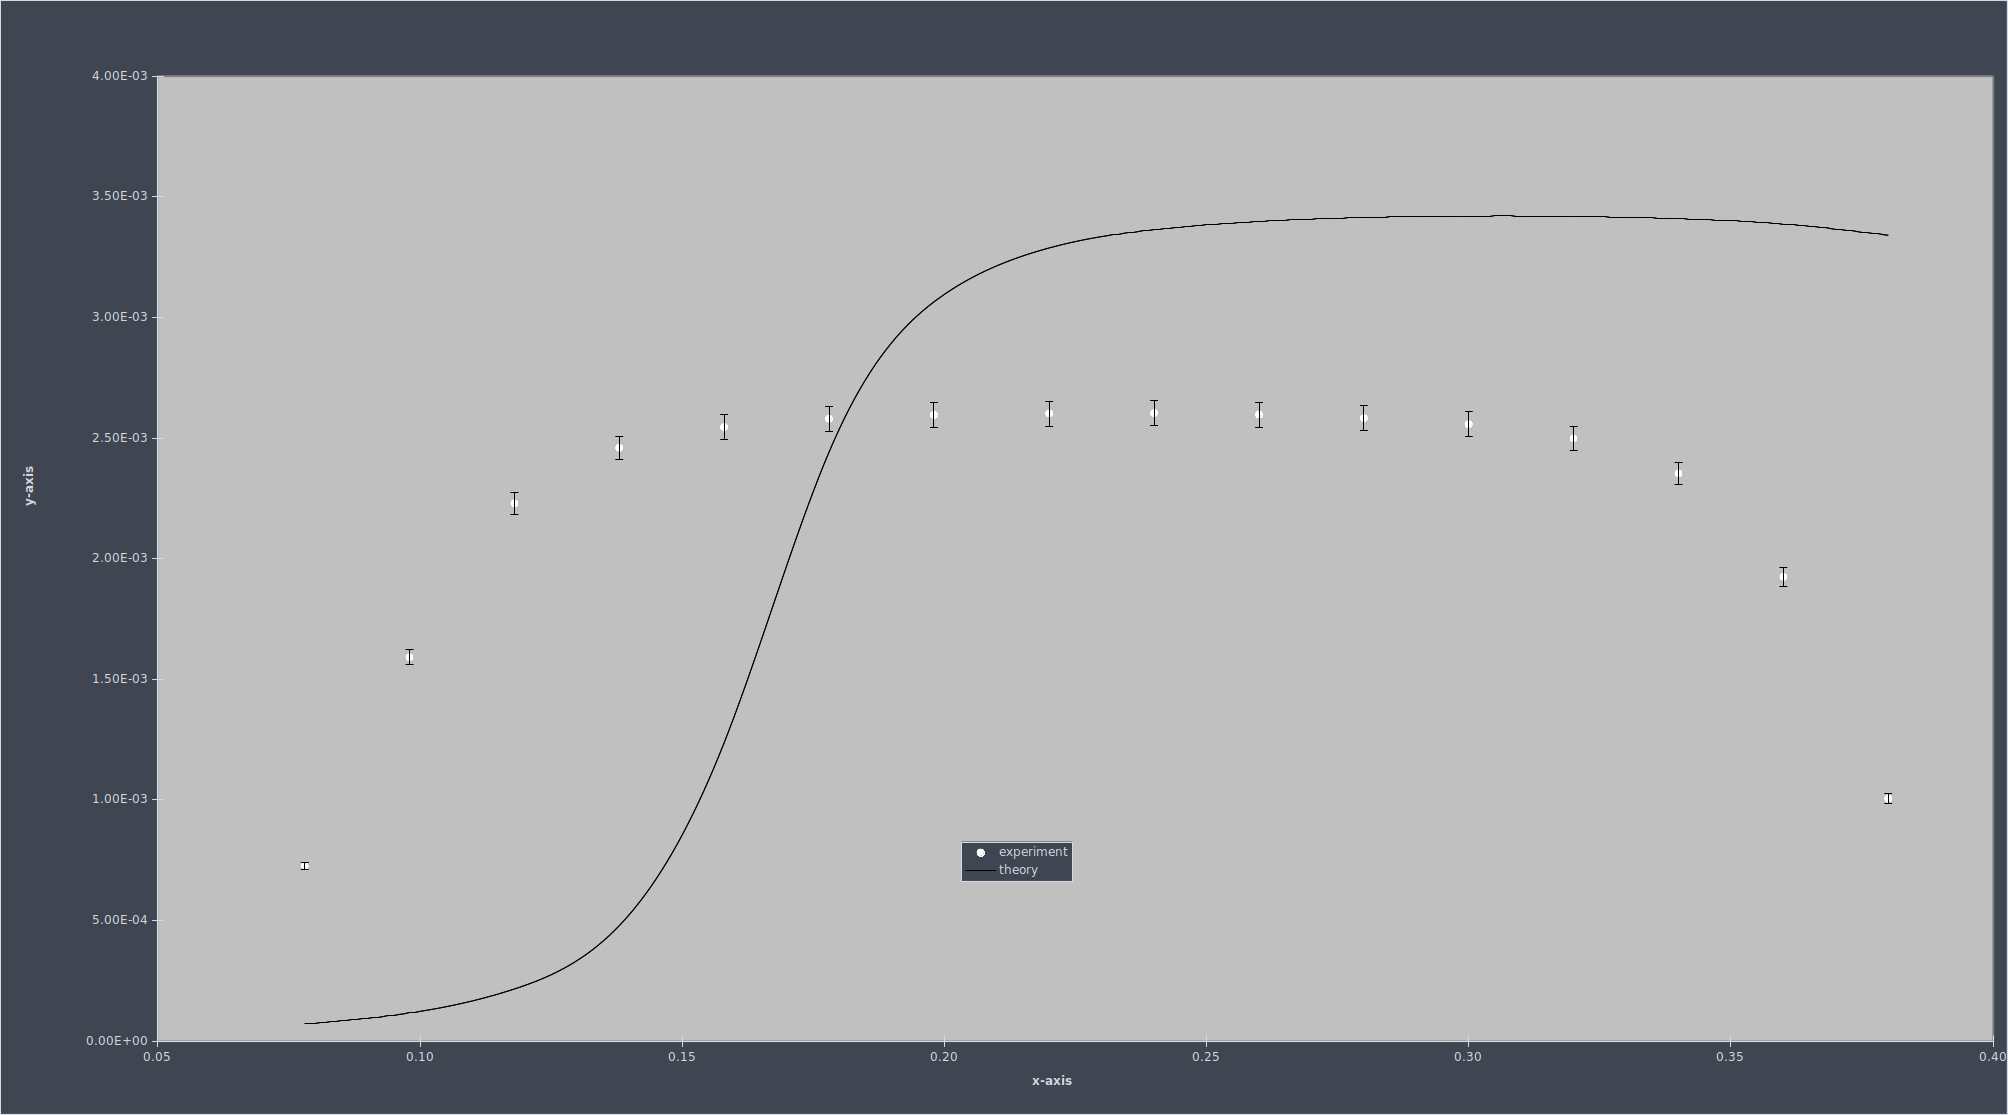
\includegraphics[width=\textwidth]{solenoid_graph.png}
    \caption{Theoretical and Measured values of $B$ (Part 1)}

\end{figure}

For part 2, Excel's LINEST function gave the following values:
\begin{itemize}
    \item The gradient was $6.29\times10^{-4}$ with an error of $1.96\times10^{-6}$
    \item An intercept of $-5.20\times10^{-4}$ was calculated too, with an error of $1.21\times10^{-6}$
\end{itemize}
Using equation \ref{eq:B_Helmholtz},
\begin{equation*}
    \begin{aligned}
        \frac{8\mu_0N}{\sqrt{125}R}                    & = 6.29\times10^{-4} \\
        N                                              & = 103.6             \\
        \Delta\left(\frac{8\mu_0N}{\sqrt{125}R}\right) & = 1.96\times10^{-6} \\
        (\Delta N)\%                                   & = 1.42\%            \\
        N                                              & = 103.6\pm1.5
    \end{aligned}
\end{equation*}
\section{Discussion}
\subsection*{Part 1}
The value of $B-B_e$ obtained was within the same order of magnitude for most of
the results, but were all slightly off from the theoretical $B_t$. This could be
due to the amplifier box being faulty, or an unset offset within the datalogging
software. Inherent inductance and resistance from the wire could be also factors,
reducing the strength of the magnetic field.
\subsection*{Part 2}
The value of $B_H$ obtained was consistent with what we expected, however an
intercept showed up when the equation was linearized. This shows that the
amplifier might not have had enough amplification on the readings, providing us
lower voltages than what might be correct values. The gradient should not have
been affected by this, and thus neither should our final result. The final value
of $N$ we obtained is in poor agreement with the theory, which might be explained
by inductance in the wire causing a reduced final magnetic field that affected the
hall effect sensor.
\section{Conclusion}
We were able to show how the magnetic field inside a solenoid stays the same
after a certain distance in, and show how the distribution varies like a bell
curve, but while the trend and distribution is similar, the values were quite
far off, around \SI{2}{\milli\tesla} from the theoretical.

For the Helmholtz coil, our value of $103\pm1.5$ was around 20 intervals away
from the theoretical value, which means that it was not consistent with the expected value.
\pagebreak
\section*{References}
\begin{itemize}
    \item 2018-2019 PHYSICS 230 Laboratory Manual (I, Isaac): Equations and Methods
    \item Cyrus Diego: Experimental results
    \item Wikipedia: Helmholtz coil and Hall effect history
\end{itemize}
\pagebreak
\section*{Appendix}
\begin{figure}[H]
    \begin{subfigure}{0.65\textwidth}
        \begin{tikzpicture}
            \begin{axis}[
                    enlargelimits=true,
                    grid=major,
                    title=$B_H$ vs $I$,
                    ylabel=$B_H$ (\si{\tesla}),
                    xlabel=$I$ (\si{\ampere}),
                    xmin=0,
                    xmax=1.0,
                    ymin=-0.00048,
                    ymax=0.00012,
                    legend entries={Data, Trendline},
                    legend pos=south east,
                    axis lines = center
                ]
                \addplot[only marks, mark=*, mark options={fill=black}] table {Lab3_2Graph.dat};
                \addplot [blue, no marks] {0.000629394*x-0.000520467};
                
            \end{axis}
        \end{tikzpicture}
        \caption{$B_H$ vs $I$ graph (Part 2)}
    \end{subfigure}
    \begin{subfigure}{0.3\textwidth}
        \begin{tabular}{|r|r|}
            \hline
            I (\si{\ampere}) & B (\si{\tesla}) \\ \hline
            0.1              & -0.000457       \\
            0.2              & -0.000398       \\
            0.3              & -0.00033        \\
            0.4              & -0.000268       \\
            0.5              & -0.000205       \\
            0.6              & -0.000141       \\
            0.7              & -8.2E-05        \\
            0.8              & -1.6E-05        \\
            0.9              & 4.6E-05         \\
            1                & 0.000108        \\ \hline
        \end{tabular}
        \caption{Recorded data (Part 2)}
    \end{subfigure}
    \caption{Part 2}
    \label{fig:part2_results}
\end{figure}
\begin{figure}[!ht]
    \begin{subfigure}{0.4\textwidth}
        \begin{tabular}{|r|r|}
            \hline
            L     & $0.280\pm0.001$\si{\meter}   \\ \hline
            R     & $0.0269\pm0.0003$\si{\meter} \\ \hline
            I     & $1\pm0.05$\si{\ampere}       \\ \hline
            $x_c$ & $0.228$\si{\meter}           \\ \hline
            $B_e$ & $-0.520$\si{\milli\tesla}    \\ \hline
        \end{tabular}
        \caption{Constants (Part 1)}
    \end{subfigure}
    \begin{subfigure}{0.5\textwidth}
        \begin{tabular}{|r|r|r|r|}
            \hline
            \thead{B                                                     \\(\si{\milli\tesla})} & \thead{Position\\(x) (\si{\meter})} & \thead{Corrected\\($B - B_e$) (\si{\tesla})} & \thead{Theoretical\\($B_t$) (\si{\tesla})} \\ \hline
            $0.207$ & $0.08$ & $7.27\times10^{-4}$ & $7.14\times10^{-5}$ \\
            $1.071$ & $0.10$ & $1.59\times10^{-3}$ & $1.17\times10^{-4}$ \\
            $1.709$ & $0.12$ & $2.23\times10^{-3}$ & $2.16\times10^{-4}$ \\
            $1.939$ & $0.14$ & $2.46\times10^{-3}$ & $4.79\times10^{-4}$ \\
            $2.025$ & $0.16$ & $2.55\times10^{-3}$ & $1.24\times10^{-3}$ \\
            $2.06$  & $0.18$ & $2.58\times10^{-3}$ & $2.44\times10^{-3}$ \\
            $2.075$ & $0.20$ & $2.60\times10^{-3}$ & $3.06\times10^{-3}$ \\
            $2.081$ & $0.22$ & $2.60\times10^{-3}$ & $3.29\times10^{-3}$ \\
            $2.083$ & $0.24$ & $2.60\times10^{-3}$ & $3.36\times10^{-3}$ \\
            $2.077$ & $0.26$ & $2.60\times10^{-3}$ & $3.40\times10^{-3}$ \\
            $2.062$ & $0.28$ & $2.58\times10^{-3}$ & $3.41\times10^{-3}$ \\
            $2.037$ & $0.30$ & $2.56\times10^{-3}$ & $3.42\times10^{-3}$ \\
            $1.978$ & $0.32$ & $2.50\times10^{-3}$ & $3.42\times10^{-3}$ \\
            $1.833$ & $0.34$ & $2.35\times10^{-3}$ & $3.41\times10^{-3}$ \\
            $1.404$ & $0.36$ & $1.92\times10^{-3}$ & $3.39\times10^{-3}$ \\
            $0.485$ & $0.38$ & $1.01\times10^{-3}$ & $3.34\times10^{-3}$ \\ \hline
        \end{tabular}
        \caption{Recorded data (Part 1)}
    \end{subfigure}
    \caption{Part 1}
    \label{fig:part1_results}
\end{figure}
\pagebreak
The expression for a single coil $B_c$ of a Helmholtz coil setup is:
\begin{equation*}
    B_c = \frac{\frac{1}{2}\mu_0NR^2I}{[R^2+(x-x_c)^2]^\frac{3}{2}}
\end{equation*}

and $N$ is the number of turns in the coil.

For the $B_s$ in the center of a solenoid, the following can be done:
\begin{equation*}
    \begin{aligned}
        B_s                    & = \frac{1}{2}\mu_0NI[\cos\beta_2-\cos\beta_1]                                                      \\
        substitute \cos\beta_2 & = \frac{x_c}{\sqrt{x_c^2 + R^2}}                                                                   \\
        and \cos\beta_1        & =\frac{L-x_c}{\sqrt{(L-x_c)^2+R^2}}                                                                \\
        B_s                    & = \frac{1}{2}\mu_0NI\left[\frac{x_c}{\sqrt{x_c^2 + R^2}}-\frac{L-x_c}{\sqrt{(L-x_c)^2+R^2}}\right] \\
                               & = \frac{\mu_0NIL}{\sqrt{L^2+4R^2}}
    \end{aligned}
\end{equation*}

where $\mu_0$ is the constant of permeability of free space, $I$ is the current
in the wire, $x$ is the current displacement from the center of the coil, $x_c$
is the displacement at the center of the coil, $R$ is the radius of the coil,
and $L$ is the length of the solenoid.

To obtain the expression for $B_H$ from $B_c$,

First obtain expression for $B_c$ at $x=R$:
\begin{equation*}
    B_c = \frac{\mu_0NIR^2}{2(R^2+(\frac{R}{2})^2)^\frac{3}{2}}
\end{equation*}
Then, multiply by two (principle of superposition for magnetic fields):
\begin{equation*}
    \begin{aligned}
        B_H = 2 B_c
         & = \frac{\mu_0NIR^2}{(R^2+(\frac{R}{2})^2)^\frac{3}{2}} \\
         & = \frac{\mu_0NIR^2}{(R^2+\frac{1}{4}R^2)^\frac{3}{2}}  \\
         & = \frac{\mu_0NIR^2}{(\frac{5}{4}R^2)^\frac{3}{2}}      \\
         & = \frac{8}{\sqrt{125}}\frac{\mu_0NIR^2}{(R^2)^\frac{3}{2}}\\
         & = \frac{8}{\sqrt{125}}\frac{\mu_0NI}{R}\\
    \end{aligned}
\end{equation*}
which is exactly equation (\ref{eq:B_Helmholtz})

\end{document}